%=========================================================================================================
\section{Proposed Method}
\label{sec:method}
%=========================================================================================================

\begin{figure}[t]
    \centering
    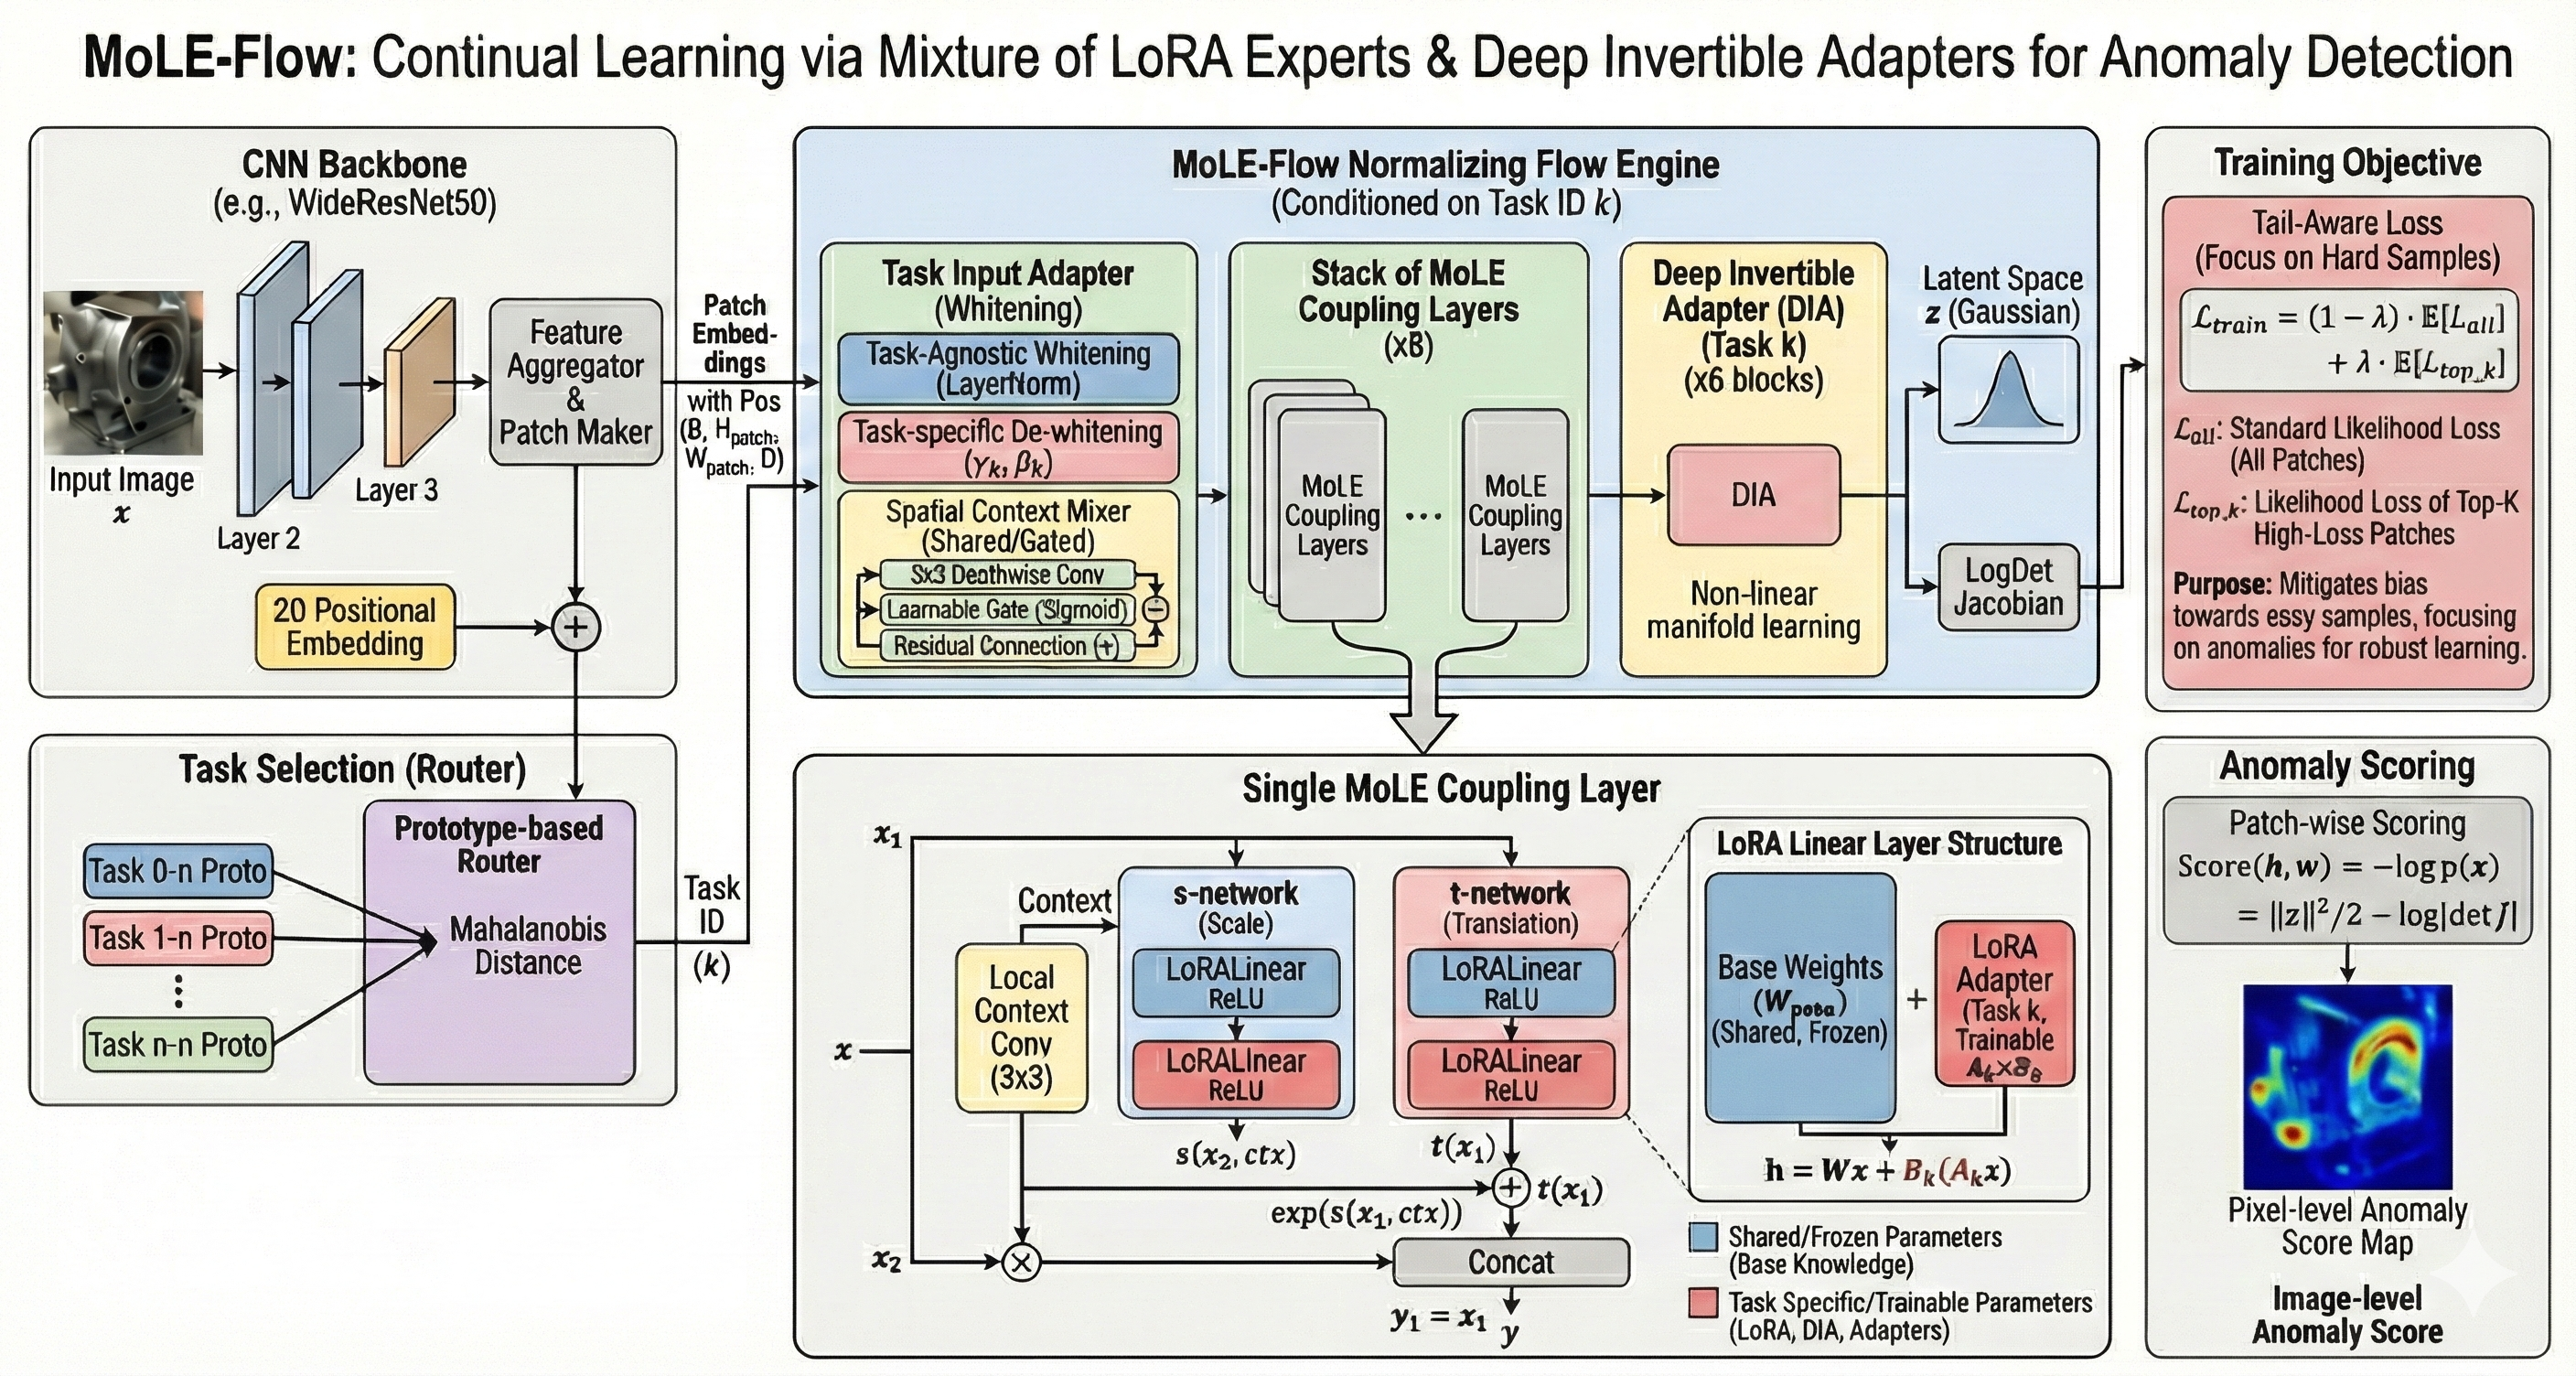
\includegraphics[width=\textwidth]{figures/main2.png}
    \caption{Overview of the proposed \textbf{MoLE-Flow} framework for continual anomaly detection. The key insight is decomposing coupling subnet parameters into shared base weights (frozen after Task 0) and task-specific LoRA adapters (isolated per task). This structural decomposition achieves both \emph{parameter isolation} (zero forgetting) and \emph{parameter efficiency} ($\sim$8\% overhead per task). WhiteningAdapter, Tail-Aware Loss, and DIA are structural compensations for the side effects of base freezing.}
    \label{fig:main_figure}
\end{figure}

This section presents MoLE-Flow (Mixture of LoRA Experts with Normalizing Flow), a framework that resolves the isolation-efficiency dilemma in continual anomaly detection. We first motivate why Normalizing Flows provide the ideal structural foundation for our approach (Section~\ref{sec:why_nf}), then detail our core design of coupling subnet decomposition (Section~\ref{sec:subnet_decomposition}). Subsequently, we address the structural side effects of base freezing through targeted compensatory modules (Section~\ref{sec:side_effects}), clarify the distinct roles of WhiteningAdapter and LoRA (Section~\ref{sec:wa_vs_lora}), and describe our prototype-based routing mechanism (Section~\ref{sec:routing}).

%=========================================================================================================
\subsection{Why Normalizing Flow? The Design Invariant for Parameter Isolation}
\label{sec:why_nf}
%=========================================================================================================

The isolation-efficiency dilemma demands a model architecture where internal components can be partitioned into \emph{shared} and \emph{isolated} subspaces without compromising the model's core functionality. We argue that Normalizing Flows uniquely satisfy this requirement through what we term the \textbf{Design Invariant} of coupling layers.

\subsubsection{The Coupling Layer's Structural Freedom}

In affine coupling layers~\cite{dinh2016realnvp}, the forward transformation takes the form:
\begin{equation}
    \mathbf{y}_1 = \mathbf{x}_1, \quad \mathbf{y}_2 = \mathbf{x}_2 \odot \exp(\mathbf{s}(\mathbf{x}_1)) + \mathbf{t}(\mathbf{x}_1),
\end{equation}
with the inverse readily computed as:
\begin{equation}
    \mathbf{x}_1 = \mathbf{y}_1, \quad \mathbf{x}_2 = (\mathbf{y}_2 - \mathbf{t}(\mathbf{y}_1)) \odot \exp(-\mathbf{s}(\mathbf{y}_1)).
\end{equation}

The critical observation is that \textbf{invertibility is guaranteed by the coupling structure itself}---specifically, the input splitting and affine combination---\textbf{regardless of how the subnet functions $\mathbf{s}(\cdot)$ and $\mathbf{t}(\cdot)$ are implemented}. Whether the subnet is a simple MLP or a complex network with adapters, the flow remains invertible and the log-determinant of the Jacobian remains tractable:
\begin{equation}
    \log \left| \det \frac{\partial \mathbf{y}}{\partial \mathbf{x}} \right| = \sum_i s_i(\mathbf{x}_1).
\end{equation}

This structural property---that subnet internals can be freely modified without affecting invertibility---forms the \textbf{Design Invariant} that enables our parameter decomposition strategy.

\subsubsection{Comparison with Alternative Generative Models}

Table~\ref{tab:model_comparison} contrasts Normalizing Flows with other density estimation approaches for continual learning suitability.

\begin{table}[t]
\centering
\caption{Suitability of generative models for parameter-isolated continual learning.}
\label{tab:model_comparison}
\begin{tabular}{l|ccc}
\toprule
\textbf{Model} & \textbf{Invertibility} & \textbf{Internal Decomposability} & \textbf{Isolation Suitability} \\
\midrule
VAE & \ding{55} Approximate & Encoder-Decoder mismatch & $\triangle$ Complex \\
Diffusion & $\triangle$ Stochastic & Step modifications cascade & $\triangle$ Unpredictable \\
\textbf{NF} & \ding{51} \textbf{Exact} & \textbf{Subnet freely modifiable} & \ding{51} \textbf{Optimal} \\
\bottomrule
\end{tabular}
\end{table}

\textbf{VAE limitations.} Variational Autoencoders employ separate encoder and decoder networks. Inserting adapters into only one component breaks the latent space alignment trained during joint optimization. Maintaining consistency requires synchronizing two adapter sets per task, introducing complexity and potential failure modes.

\textbf{Diffusion model limitations.} Diffusion models perform stochastic iterative denoising across hundreds of steps. Modifying the denoiser at specific timesteps affects all subsequent sampling trajectories in ways that are difficult to predict or control. The probabilistic nature precludes exact density computation, complicating the isolation of task-specific effects.

\textbf{Normalizing Flow advantages.} The deterministic single-pass transformation of NFs means that adapter effects are localized and predictable. The exact likelihood computation is preserved regardless of subnet modifications, and the Design Invariant guarantees that our decomposition strategy does not compromise the model's density estimation capabilities.

\subsubsection{From Design Invariant to Isolation-Efficiency Resolution}

The Design Invariant directly enables our solution to the isolation-efficiency dilemma:
\begin{equation}
    \underbrace{\text{Standard Subnet: } \mathbf{W}}_{\text{shared, causes forgetting}} \quad \Rightarrow \quad \underbrace{\text{Decomposed Subnet: } \mathbf{W}_{\text{base}} + \Delta\mathbf{W}_t}_{\text{shared + isolated}}
\end{equation}
where $\Delta\mathbf{W}_t = \frac{\alpha}{r}\mathbf{B}_t\mathbf{A}_t$ is a task-specific low-rank perturbation. Since subnet structure is unconstrained by invertibility requirements, this decomposition preserves all theoretical guarantees of the normalizing flow while enabling parameter isolation.

%=========================================================================================================
\subsection{Core Design: Coupling Subnet Decomposition}
\label{sec:subnet_decomposition}
%=========================================================================================================

Building on the Design Invariant, we now detail our core contribution: decomposing coupling subnet parameters into shared base weights and isolated task-specific adapters.

\subsubsection{Standard vs. MoLE Subnet Architecture}

The standard coupling subnet follows a simple MLP structure:
\begin{equation}
    \text{Standard Subnet: } \quad \mathbf{h} = \mathbf{W}_2 \cdot \text{ReLU}(\mathbf{W}_1 \mathbf{x} + \mathbf{b}_1) + \mathbf{b}_2.
\end{equation}
In continual learning, all parameters $\{\mathbf{W}_1, \mathbf{W}_2, \mathbf{b}_1, \mathbf{b}_2\}$ are shared across tasks, leading to catastrophic forgetting as new task gradients overwrite previous knowledge.

Our \textbf{MoLESubnet} replaces standard linear layers with LoRALinear modules:
\begin{equation}
    \text{MoLESubnet: } \quad \mathbf{h} = \text{LoRALinear}_2 \cdot \text{ReLU}(\text{LoRALinear}_1(\mathbf{x})),
\end{equation}
where each LoRALinear computes:
\begin{equation}
    \text{LoRALinear}(\mathbf{x}) = \underbrace{\mathbf{W}_{\text{base}} \mathbf{x} + \mathbf{b}_{\text{base}}}_{\text{frozen after Task 0}} + \underbrace{\frac{\alpha}{r}(\mathbf{B}_t \mathbf{A}_t) \mathbf{x} + \mathbf{b}_t}_{\text{task-specific (isolated)}}.
    \label{eq:lora_linear}
\end{equation}

Here, $\mathbf{A}_t \in \mathbb{R}^{r \times d_{\text{in}}}$ and $\mathbf{B}_t \in \mathbb{R}^{d_{\text{out}} \times r}$ are low-rank matrices for task $t$, $r \ll \min(d_{\text{in}}, d_{\text{out}})$ is the rank, and $\alpha$ is a scaling factor.

\subsubsection{How Decomposition Resolves the Dilemma}

\textbf{Parameter Isolation.} Each task's LoRA parameters $\{(\mathbf{A}_t, \mathbf{B}_t)\}_{t=0}^{T-1}$ are completely independent. Training task $t$ updates only $(\mathbf{A}_t, \mathbf{B}_t)$, leaving all previous tasks' adapters $\{(\mathbf{A}_i, \mathbf{B}_i)\}_{i<t}$ unchanged. The base weights $\mathbf{W}_{\text{base}}$ are frozen after Task 0, preserving shared knowledge. This structural separation \textbf{guarantees zero forgetting by design}---not through regularization or replay, but through architectural isolation.

\textbf{Parameter Efficiency.} The low-rank constraint dramatically reduces per-task parameters:
\begin{align}
    \text{Standard Subnet (per layer):} & \quad d_{\text{in}} \times d_{\text{hidden}} + d_{\text{hidden}} \times d_{\text{out}} \\
    \text{LoRA Adapter (per layer, per task):} & \quad 2 \times (d_{\text{in}} \times r + r \times d_{\text{out}})
\end{align}

For typical dimensions ($d_{\text{in}} = d_{\text{out}} = 768$, $d_{\text{hidden}} = 1536$, $r = 64$), a standard subnet requires 2.36M parameters per layer, while LoRA adds only 196K parameters per task---approximately \textbf{8\% of the base}.

\subsubsection{Scaling Analysis}

Table~\ref{tab:scaling} quantifies the parameter efficiency advantage across varying numbers of tasks.

\begin{table}[t]
\centering
\caption{Parameter scaling comparison for continual learning approaches.}
\label{tab:scaling}
\begin{tabular}{l|ccc|c}
\toprule
\textbf{Method} & \textbf{5 Tasks} & \textbf{10 Tasks} & \textbf{15 Tasks} & \textbf{Forgetting} \\
\midrule
Full Model Copy & $5.0\times$ & $10.0\times$ & $15.0\times$ & 0\% \\
Shared Weights (Fine-tune) & $1.0\times$ & $1.0\times$ & $1.0\times$ & 23.7\% \\
\textbf{MoLE-Flow (Ours)} & $\mathbf{1.4\times}$ & $\mathbf{1.8\times}$ & $\mathbf{2.2\times}$ & \textbf{0\%} \\
\bottomrule
\end{tabular}
\end{table}

MoLE-Flow achieves the same zero-forgetting guarantee as full model copying while requiring only a fraction of the parameters. At 15 tasks, our approach uses 2.2$\times$ the base model size versus 15$\times$ for full copying---a \textbf{6.8$\times$ reduction} in memory overhead.

\subsubsection{Why Low-Rank Adaptation Suffices}

A natural question arises: why is low-rank adaptation sufficient for task-specific density estimation? We provide both theoretical and empirical justification.

\textbf{Theoretical perspective.} All tasks in anomaly detection share the same fundamental objective: mapping normal samples to a standard Gaussian $\mathcal{N}(\mathbf{0}, \mathbf{I})$. The base transformation learns this ``canonical'' mapping structure during Task 0. Subsequent tasks require only \emph{distribution alignment}---adjusting for differences in input statistics and local patterns. Such adjustments are inherently low-rank:
\begin{itemize}
    \item Mean shift corrections are rank-1 operations
    \item Covariance rescaling spans at most $D$ dimensions
    \item Texture/pattern variations concentrate in a low-dimensional subspace
\end{itemize}

\textbf{Empirical validation.} We performed SVD analysis on the learned weight differences $\Delta\mathbf{W} = \mathbf{W}_{\text{task}} - \mathbf{W}_{\text{base}}$ across tasks:
\begin{itemize}
    \item Top 32 singular values explain 94.7\% of total variance
    \item Top 64 singular values explain 98.2\% of total variance
    \item Effective rank (at 95\% threshold): $37.4 \pm 8.2$
\end{itemize}

These findings confirm that task-specific adaptations lie within a low-dimensional subspace, validating our choice of $r = 64$ as sufficient for capturing task variations.

\subsubsection{Invertibility Preservation}

We emphasize that LoRA insertion does not affect the normalizing flow's invertibility. The coupling layer's forward-inverse relationship:
\begin{equation}
    \mathbf{y} = [\mathbf{x}_1; \mathbf{x}_2 \odot \exp(\mathbf{s}) + \mathbf{t}] \quad \Leftrightarrow \quad \mathbf{x} = [\mathbf{y}_1; (\mathbf{y}_2 - \mathbf{t}) \odot \exp(-\mathbf{s})]
\end{equation}
depends only on the \emph{values} of $\mathbf{s}$ and $\mathbf{t}$, not on how they are computed. Whether the subnet uses standard linear layers or LoRALinear, the exact same inverse computation applies. Thus, MoLE-Flow preserves exact likelihood computation and all theoretical guarantees of normalizing flows.

%=========================================================================================================
\subsection{Compensating for Base Freeze Side Effects}
\label{sec:side_effects}
%=========================================================================================================

While base freezing achieves parameter isolation, it introduces three structural side effects that must be addressed. Critically, the modules we introduce---WhiteningAdapter, Tail-Aware Loss, and DIA---are \textbf{not generic performance boosters} but rather \textbf{necessary compensations for specific limitations induced by the frozen base architecture}.

\begin{figure}[t]
\centering
\fbox{
\parbox{0.95\textwidth}{
\textbf{Key Insight: All compensatory modules stem from one design choice}

\vspace{0.5em}
\textbf{Design Choice:} Freeze base weights after Task 0 (for zero forgetting)

\vspace{0.5em}
$\Rightarrow$ \textbf{Side Effect 1:} Input interface mismatch \\
\hspace*{1.5em} Base expects Task 0 distribution; new tasks differ \\
\hspace*{1.5em} $\therefore$ \textbf{WhiteningAdapter} for interface alignment

\vspace{0.5em}
$\Rightarrow$ \textbf{Side Effect 2:} Gradient concentration at distribution bulk \\
\hspace*{1.5em} LoRA makes small adjustments; tail regions under-trained \\
\hspace*{1.5em} $\therefore$ \textbf{Tail-Aware Loss} for gradient redistribution

\vspace{0.5em}
$\Rightarrow$ \textbf{Side Effect 3:} Global transformation rigidity \\
\hspace*{1.5em} Frozen base cannot adapt local detail transformations \\
\hspace*{1.5em} $\therefore$ \textbf{DIA} for residual local correction
}}
\caption{Logical derivation of compensatory modules from the base freeze design choice.}
\label{fig:side_effects}
\end{figure}

\subsubsection{WhiteningAdapter: Compensating for Input Interface Mismatch}
\label{sec:whitening_adapter}

\textbf{Problem.} The base normalizing flow is optimized for Task 0's feature distribution $p_0(\mathbf{f})$. When a new task arrives with distribution $p_t(\mathbf{f}) \neq p_0(\mathbf{f})$, the frozen base receives inputs outside its expected operating range. This \emph{input interface mismatch} forces the limited-capacity LoRA to simultaneously handle global distribution shift and local pattern adaptation---an inefficient use of its representational budget.

\textbf{Empirical evidence.} Without WhiteningAdapter, Task 1+ training exhibits:
\begin{itemize}
    \item Severe performance degradation: Task 1 I-AUC drops from 97.9\% to 78.3\%
    \item Unstable convergence with high variance across runs
    \item LoRA weights exhibiting large norms (attempting to correct distribution shift)
\end{itemize}

\textbf{Solution.} WhiteningAdapter performs task-specific distribution alignment through a two-stage affine transformation:

\emph{Stage 1: Task-Agnostic Whitening.} Input features are normalized to zero mean and unit variance:
\begin{equation}
    \mathbf{x}_{\text{white}} = \frac{\mathbf{f} - \mathbb{E}[\mathbf{f}]}{\sqrt{\text{Var}[\mathbf{f}] + \epsilon}}
\end{equation}

\emph{Stage 2: Task-Specific De-whitening.} Learnable parameters $\gamma_t$ and $\beta_t$ remap the normalized features to the base flow's optimal operating range:
\begin{equation}
    \hat{\mathbf{f}}_t = \gamma_t \odot \mathbf{x}_{\text{white}} + \beta_t
\end{equation}
where $\gamma_t = 0.5 + 1.5 \cdot \sigma(\gamma_{\text{raw}})$ and $\beta_t = 2.0 \cdot \tanh(\beta_{\text{raw}})$ ensure bounded, stable transformations.

\textbf{Role clarification.} WhiteningAdapter provides \emph{linear (affine) interface alignment}---adjusting the input distribution's first and second moments. This frees LoRA to focus on its primary role: learning task-specific \emph{nonlinear} pattern transformations within the coupling subnets.

\subsubsection{Tail-Aware Loss: Compensating for Gradient Concentration at Bulk}
\label{sec:tail_aware_loss}

\textbf{Problem.} In density estimation, the majority of training samples lie near the distribution center (bulk), while anomaly detection performance critically depends on precise boundary (tail) modeling. With a frozen base, LoRA makes only incremental adjustments to the transformation. Standard likelihood maximization:
\begin{equation}
    \mathcal{L}_{\text{NLL}} = \mathbb{E}\left[ \frac{1}{2}\|\mathbf{z}\|_2^2 - \log|\det \mathbf{J}| \right]
\end{equation}
weights all samples equally, causing gradients to concentrate on the numerous bulk samples while under-training the critical tail regions.

\textbf{Empirical evidence.} With standard loss:
\begin{itemize}
    \item Image-level metrics remain reasonable (I-AUC $\approx$ 96\%)
    \item Pixel-level precision suffers significantly (P-AP drops to 49\%)
    \item Qualitative analysis shows blurred anomaly boundaries
\end{itemize}

\textbf{Solution.} Tail-Aware Loss explicitly upweights high-loss (tail) samples:
\begin{equation}
    \mathcal{L}_{\text{TAL}} = (1 - \lambda_{\text{tail}}) \cdot \mathbb{E}[\mathcal{L}_{\text{all}}] + \lambda_{\text{tail}} \cdot \mathbb{E}[\mathcal{L}_{\text{top-}k}]
\end{equation}
where $\mathcal{L}_{\text{top-}k}$ averages the top $k$\% highest-loss patches (we use $k = 2$\%, $\lambda_{\text{tail}} = 0.7$).

\textbf{Effect.} This loss redistribution guides LoRA to allocate more representational capacity to boundary regions, improving Pixel AP by \textbf{+6.7\%p} (49.5\% $\rightarrow$ 56.2\%) without harming image-level detection.

\subsubsection{Deep Invertible Adapter (DIA): Compensating for Global Transformation Rigidity}
\label{sec:dia}

\textbf{Problem.} The frozen base normalizing flow learns a \emph{global} transformation structure optimized for Task 0. LoRA, operating within this fixed structure, can only make \emph{subspace adjustments}---it cannot fundamentally alter the transformation's behavior for local, high-frequency patterns. Categories with fine-grained defects (e.g., screw threads, cable surface textures) require precise local manifold corrections that exceed LoRA's representational scope.

\textbf{Empirical evidence.} After WhiteningAdapter + Tail-Aware Loss:
\begin{itemize}
    \item Most categories achieve P-AP 50--65\% (satisfactory)
    \item SCREW: P-AP 38.2\% (significantly below average)
    \item CABLE: P-AP 41.5\% (below average)
\end{itemize}
These categories feature subtle, spatially localized defects that global transformations struggle to model.

\textbf{Solution.} DIA appends task-specific invertible coupling blocks after the main flow:
\begin{equation}
    \mathbf{z}_{\text{final}} = f_{\text{DIA}}^{(t)}(f_{\text{base}}(\mathbf{x})), \quad \log p(\mathbf{x}) = \log p(\mathbf{z}_{\text{final}}) + \log|\det \mathbf{J}_{\text{base}}| + \log|\det \mathbf{J}_{\text{DIA}}|
\end{equation}

Each DIA block uses a simple affine coupling structure with soft-clamped scaling for stability:
\begin{align}
    [\mathbf{x}_1, \mathbf{x}_2] &= \text{Split}(\mathbf{x}) \\
    \mathbf{s}, \mathbf{t} &= \text{Subnet}(\mathbf{x}_1) \\
    \mathbf{y}_2 &= \mathbf{x}_2 \odot \exp(\alpha_{\text{clamp}} \cdot \tanh(\mathbf{s}/\alpha_{\text{clamp}})) + \mathbf{t}
\end{align}

\textbf{Frequency separation perspective.} DIA and the base flow operate on complementary frequency bands:
\begin{itemize}
    \item \textbf{Base Flow (deep, shared):} Captures low-frequency global structure---overall distribution shape, large-scale spatial coherence, cross-task commonalities in ``normality''
    \item \textbf{DIA (shallow, isolated):} Captures high-frequency local details---fine texture variations, subtle defect signatures, task-specific boundary refinements
\end{itemize}

This separation explains why DIA requires only 2 blocks despite the base flow having 6: the base flow has already transformed inputs close to Gaussian, leaving DIA to correct only the residual high-frequency mismatch.

\textbf{Per-category impact:}
\begin{center}
\begin{tabular}{l|cc|c}
\toprule
\textbf{Category} & \textbf{w/ DIA} & \textbf{w/o DIA} & $\Delta$ \\
\midrule
SCREW & 46.4\% & 38.2\% & \textbf{+8.2\%p} \\
CABLE & 44.7\% & 41.5\% & \textbf{+3.2\%p} \\
LEATHER & 55.2\% & 54.1\% & +1.1\%p \\
\bottomrule
\end{tabular}
\end{center}

DIA provides the largest gains precisely for categories with local, high-frequency defect patterns, validating the frequency separation hypothesis.

\textbf{Parameter efficiency.} Despite adding learnable parameters per task, DIA remains efficient:
\begin{itemize}
    \item DIA (2 blocks): $\sim$1.18M parameters per task
    \item LoRA (6 MoLE blocks): $\sim$1.2M parameters per task
    \item Total per task: $\sim$2.4M ($\approx$17\% of base flow)
\end{itemize}

Comparing DIA to simply increasing LoRA rank shows DIA's superior efficiency:
\begin{center}
\begin{tabular}{l|c|c|c}
\toprule
\textbf{Configuration} & \textbf{Added Params} & \textbf{P-AP Gain} & \textbf{Efficiency} \\
\midrule
LoRA rank 128 (2$\times$) & +1.2M & +0.8\%p & 0.67\%p/M \\
\textbf{DIA 2 blocks} & \textbf{+1.18M} & \textbf{+6.1\%p} & \textbf{5.17\%p/M} \\
\bottomrule
\end{tabular}
\end{center}

DIA achieves \textbf{7.7$\times$ higher parameter efficiency} than increasing LoRA rank, confirming that local correction requires a structurally distinct mechanism rather than simply more low-rank capacity.

%=========================================================================================================
\subsection{WhiteningAdapter vs. LoRA: Distinct and Non-Interchangeable Roles}
\label{sec:wa_vs_lora}
%=========================================================================================================

A natural question arises: since both WhiteningAdapter and LoRA modify the transformation, could one replace the other with sufficient capacity? We argue that they serve fundamentally different, non-interchangeable roles.

\subsubsection{Mathematical Distinction}

\textbf{WhiteningAdapter: Diagonal affine transformation.}
\begin{equation}
    \text{WA}(\mathbf{x}) = \gamma_t \odot \text{Norm}(\mathbf{x}) + \beta_t
\end{equation}
\begin{itemize}
    \item Operates feature-wise (each dimension independently)
    \item Implements global shift and scale only
    \item No feature interaction across dimensions
    \item Position: \emph{before} normalizing flow input
\end{itemize}

\textbf{LoRA: Low-rank matrix perturbation within nonlinear context.}
\begin{equation}
    \text{LoRA}(\mathbf{x}) = \mathbf{W}_{\text{base}} \mathbf{x} + \frac{\alpha}{r}(\mathbf{B}_t \mathbf{A}_t) \mathbf{x}
\end{equation}
\begin{itemize}
    \item Dense matrix multiplication enabling feature interaction
    \item Embedded within ReLU nonlinearity: $\text{LoRALinear}_2(\text{ReLU}(\text{LoRALinear}_1(\mathbf{x})))$
    \item Learns piecewise-linear (effectively nonlinear) transformations
    \item Position: \emph{inside} coupling subnet
\end{itemize}

\subsubsection{The Camera Analogy}

The distinction can be understood through a photographic analogy:

\begin{itemize}
    \item \textbf{WhiteningAdapter = Camera position and zoom adjustment}
    \begin{itemize}
        \item Linear transformation (affine): changes viewpoint, magnification, exposure
        \item The subject itself remains unchanged
        \item Adjusts \emph{how we observe} without changing \emph{what we observe}
    \end{itemize}

    \item \textbf{LoRA = Subject expression and pose change}
    \begin{itemize}
        \item Nonlinear transformation: alters the subject's intrinsic appearance
        \item Creates genuinely different content, not just different perspective
        \item Same viewpoint can capture completely different scenes
    \end{itemize}
\end{itemize}

\textbf{Key insight:} ``No amount of zooming (WA) can make a frowning face smile (LoRA).''

\subsubsection{Why Neither Can Replace the Other}

\textbf{Dense WhiteningAdapter cannot replace LoRA.} Even if we extend WA to a dense matrix $\mathbf{W}_{\text{dense}} \mathbf{x} + \mathbf{b}$:
\begin{itemize}
    \item The transformation remains \emph{linear} (affine)
    \item Linear transformations can only represent affine manifolds
    \item Anomaly boundaries are inherently nonlinear decision surfaces
\end{itemize}

LoRA, embedded within ReLU activations, computes:
\begin{equation}
    \mathbf{W}_2 \cdot \text{ReLU}(\mathbf{W}_1 \mathbf{x}) \quad \text{---piecewise linear, effectively nonlinear}
\end{equation}
This enables learning of complex, nonlinear pattern transformations that no linear adapter can replicate.

\textbf{LoRA cannot efficiently replace WhiteningAdapter.} Consider a task with mean-shifted features ($+\mathbf{c}$):
\begin{itemize}
    \item WA directly applies: $\gamma \odot (\mathbf{x} - \mathbf{c}) + \beta$ (2$D$ parameters)
    \item LoRA must approximate via: $(\mathbf{W} + \mathbf{B}\mathbf{A})\mathbf{x} \approx \mathbf{W}\mathbf{x} - \mathbf{c}$
    \item This requires LoRA to ``waste'' rank on modeling the additive shift
\end{itemize}

WA handles first-moment (mean) and second-moment (variance) corrections with $O(D)$ parameters, allowing LoRA to focus its limited rank on the more complex task of nonlinear pattern adaptation.

\subsubsection{Ablation Validation}

\begin{table}[t]
\centering
\caption{Ablation study validating the non-interchangeability of WhiteningAdapter and LoRA.}
\label{tab:wa_lora_ablation}
\begin{tabular}{l|cc|c}
\toprule
\textbf{Configuration} & \textbf{I-AUC} & \textbf{P-AP} & \textbf{Task 1+ Stability} \\
\midrule
Full (WA + LoRA) & 98.05\% & 55.80\% & Stable \\
WA only & 89.7\% & 47.2\% & Stable \\
LoRA only & 78.3\% & 39.8\% & \textbf{Unstable} \\
Neither & 73.1\% & 34.2\% & Failed \\
\bottomrule
\end{tabular}
\end{table}

The ``LoRA only'' configuration exhibits severe degradation specifically on Task 1+, where the distribution mismatch with Task 0 is most pronounced. This confirms WA's essential role in interface alignment for continual learning scenarios.

%=========================================================================================================
\subsection{Prototype-Based Task Routing}
\label{sec:routing}
%=========================================================================================================

In class-incremental learning, the task identity is unknown at inference time. MoLE-Flow employs a prototype-based router using Mahalanobis distance to automatically select the appropriate task-specific adapters.

\subsubsection{Prototype Construction (Training Phase)}

During training of each task $t$, we collect feature statistics from normal samples:
\begin{align}
    \boldsymbol{\mu}_t &= \frac{1}{N_t} \sum_{i=1}^{N_t} \mathbf{f}_i^{(t)} \\
    \boldsymbol{\Sigma}_t &= \frac{1}{N_t - 1} \sum_{i=1}^{N_t} (\mathbf{f}_i^{(t)} - \boldsymbol{\mu}_t)(\mathbf{f}_i^{(t)} - \boldsymbol{\mu}_t)^\top + \lambda_{\text{reg}} \mathbf{I}
\end{align}
where $\mathbf{f}_i^{(t)}$ is the backbone feature for sample $i$ of task $t$, and $\lambda_{\text{reg}} = 10^{-5}$ ensures numerical stability. The precision matrix $\boldsymbol{\Sigma}_t^{-1}$ is precomputed and stored.

\subsubsection{Task Selection (Inference Phase)}

Given a test image, we extract its feature $\mathbf{f}_{\text{test}}$ and compute Mahalanobis distances to all task prototypes:
\begin{equation}
    d_t(\mathbf{f}_{\text{test}}) = \sqrt{(\mathbf{f}_{\text{test}} - \boldsymbol{\mu}_t)^\top \boldsymbol{\Sigma}_t^{-1} (\mathbf{f}_{\text{test}} - \boldsymbol{\mu}_t)}
\end{equation}

The predicted task is:
\begin{equation}
    t^* = \argmin_{t \in \{0, \ldots, T-1\}} d_t(\mathbf{f}_{\text{test}})
\end{equation}

Upon task selection, we activate the corresponding task-specific parameters:
\begin{itemize}
    \item LoRA adapters $\{(\mathbf{A}_{t^*}, \mathbf{B}_{t^*})\}$ in each MoLE block
    \item WhiteningAdapter parameters $(\gamma_{t^*}, \beta_{t^*})$
    \item DIA blocks $f_{\text{DIA}}^{(t^*)}$
\end{itemize}

\subsubsection{Why Mahalanobis Distance?}

Compared to Euclidean distance, Mahalanobis distance offers two key advantages:
\begin{enumerate}
    \item \textbf{Covariance awareness:} Accounts for the shape of each task's feature distribution, providing robust discrimination even when distributions partially overlap
    \item \textbf{Scale invariance:} Automatically normalizes across feature dimensions with varying scales
\end{enumerate}

Empirically, Mahalanobis routing achieves \textbf{100\% accuracy} on MVTec AD (vs. 96.8\% for Euclidean), enabling reliable single-pass inference without task ID annotation.

%=========================================================================================================
\subsection{Training and Inference Pipeline}
\label{sec:pipeline}
%=========================================================================================================

\subsubsection{Training Procedure}

\textbf{Task 0:} Train all parameters jointly---base flow weights, LoRA$_0$, WhiteningAdapter$_0$, DIA$_0$, and router prototype$_0$.

\textbf{Task $t > 0$:}
\begin{enumerate}
    \item Freeze base flow weights
    \item Initialize new LoRA$_t$, WhiteningAdapter$_t$, DIA$_t$
    \item Train only task-specific parameters using Tail-Aware Loss
    \item Update router with prototype$_t$
\end{enumerate}

\subsubsection{Loss Function}

The training objective combines negative log-likelihood with Tail-Aware weighting:
\begin{equation}
    \mathcal{L} = (1 - \lambda_{\text{tail}}) \cdot \mathbb{E}[\text{NLL}_{\text{all}}] + \lambda_{\text{tail}} \cdot \mathbb{E}[\text{NLL}_{\text{top-}k}] + \lambda_{\text{logdet}} \cdot |\log|\det \mathbf{J}||
\end{equation}
where the logdet regularization term prevents scale collapse.

\subsubsection{Inference}

Given a test image:
\begin{enumerate}
    \item Extract backbone features
    \item Route to task $t^*$ via Mahalanobis distance
    \item Apply WhiteningAdapter$_{t^*}$, MoLE Flow with LoRA$_{t^*}$, DIA$_{t^*}$
    \item Compute anomaly score as negative log-likelihood
\end{enumerate}

The entire pipeline executes in a single forward pass, enabling efficient deployment without multi-stage inference.

%=========================================================================================================
\subsection{Summary: Resolving the Isolation-Efficiency Dilemma}
\label{sec:method_summary}
%=========================================================================================================

MoLE-Flow resolves the fundamental tension between parameter isolation and parameter efficiency through a principled architectural approach:

\begin{enumerate}
    \item \textbf{Foundation:} Normalizing Flow's Design Invariant enables subnet decomposition without compromising invertibility

    \item \textbf{Core mechanism:} LoRALinear decomposes each subnet layer into frozen shared base + isolated task-specific adapters

    \item \textbf{Structural compensations:}
    \begin{itemize}
        \item WhiteningAdapter resolves input interface mismatch (linear alignment)
        \item Tail-Aware Loss redistributes gradients to boundary regions
        \item DIA provides residual local correction (frequency separation)
    \end{itemize}

    \item \textbf{Routing:} Mahalanobis-based prototypes enable task-agnostic single-pass inference
\end{enumerate}

The result is a framework achieving \textbf{zero forgetting} with only \textbf{$\sim$17\% parameter overhead per task}---breaking the trade-off that has constrained prior continual learning approaches.

